\section{Funktionen des Systems}
Um die benötigten Funktionen unseres System zu eruieren, wird der Ablauf des gesamten Systems bildlich dargestellt. Der Ablauf startet bereits mit einem Startsignal und endet mit dem Stoppsignal.

\begin{figure}[h!]
\centering
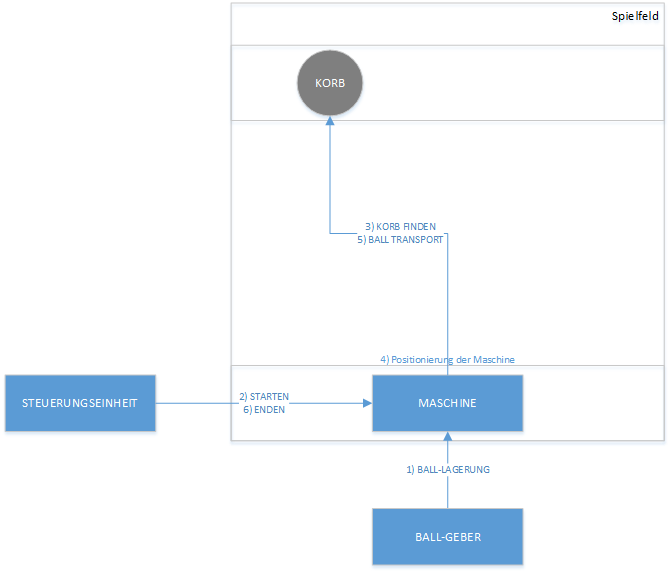
\includegraphics[width=0.7\linewidth]{../../fig/ablauf-transport}
\caption[Gesamter Ablauf des Transports]{Gesamter Ablauf des Transports}
\label{fig:ablauf-transport}
\end{figure}

Auf der Abbildung \ref{fig:ablauf-transport} sind die einzelnen Schritte zu erkennen, welche durchlaufen werden müssen. Die Nummerierung stellt die Reihenfolge dar. Die STEUERUNGSEINHEIT ist eine externe Einheit, welche mit der MASCHINE kommuniziert. Die MASCHINE ist dann für den eigentlichen Transport der Bälle verantwortlich. Die Aktion des BALL-GEBER kann eine manuelle Interaktion mit der MASCHINE sein.\\
\\
Im ersten Schritt übergibt der BALL-GEBER die Bälle der Maschine, darauf folgt ein Startsignal der STEUERUNGSEINHEIT. Anschliessend muss die MASCHINE den Korb im Spielfeld orten und sich im Schritt 4 entsprechend positionieren. Nach dem Transport der Bälle sendet die MASCHINE ein Stopsignal an die STEUERUNGSEINHEIT.

\subsection{Funktionen}
Aus diesen Aktivitäten lassen sich die Funktionen ableiten, welche das System leisten muss:\\
 
\emph{Ball-Lagerung}\\
Der Ball-Geber übergibt im Schritt 1 der Maschine die Bälle. Die Bälle müssen danach von der Maschine gelagert werden.\\
\\
\emph{Kommunikation}\\
Die Steuerungseinheit und die Maschine müssen in den Schritten 2 und 6 miteinander kommunizieren.\\
\\
\emph{Ortung des Korbs}\\
Im Schritt 3 muss der Korb geortet werden.\\
\\
\emph{Maschinen Positionierung}\\
Die Maschine muss im Schritt 4 positioniert werden. Das ist unabhängig davon ob die gesamte Maschine die Position ändert oder ob die Maschine mechanische Teile bewegt.\\
\\
\emph{Transport der Bälle}\\
Im vorletzten Schritt werden die Bälle in den Korb transportiert.\\
\\
\emph{Energieversorgung}\\
Dieser Punkt lässt sich nicht direkt aus dem Ablauf erkennen. Jedoch ist diese Funktion zentral, denn die Steuerungseinheit und auch die Maschine müssen mit Energie versorgt werden. Daher wird dieser Punkt explizit aufgenommen.\\
\\\emph{Computer}\\
Auch dieser Punkt ist sehr wichtig und nicht direkt ableitbar aus dem Ablauf. Die Maschine und auch die Steuerungseinheit müssen möglicherweise Berechnung vornehmen.